\documentclass{article}
\usepackage{graphicx}
\usepackage{subfig}
    
\begin{document}

\begin{figure}[htbp]
    \centering
    \fbox{
        \subfloat[doraemon (1)\label{7.1}]{

            \fbox{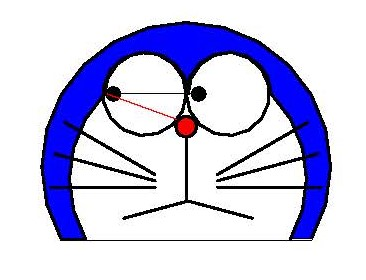
\includegraphics[width=.25\textwidth]{doraemon1.jpg}}
        }
    }
    \hfill
    \fbox{
        \subfloat[doraemon (2)\label{7.2}]{

            \fbox{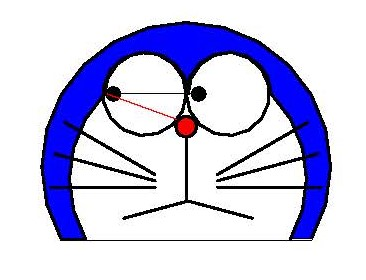
\includegraphics[width=.25\textwidth]{doraemon1.jpg}}
        }
    }
    \hfill
    \fbox{
        \subfloat[doraemon (3)]{
            \label{7.3} %* "\label{}"命令既可以放在可选参数内,也可以放在必选参数内
            \fbox{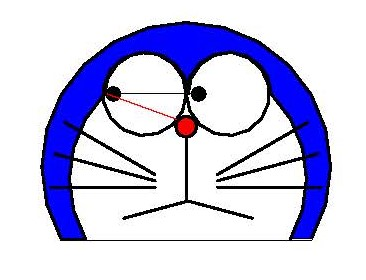
\includegraphics[width=.25\textwidth]{doraemon1.jpg}}
        }
    }
    \caption{doraemon\_subfig\_subfloat}
    \label{7}
\end{figure}

    
\begin{figure}[htbp]
    \centering
    \fbox{
        \subfloat[doraemon (1)]{
            \fbox{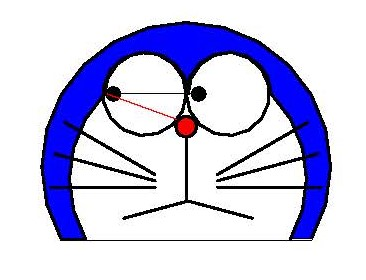
\includegraphics[scale=.1]{doraemon1.jpg}}
        }
    }
    \hfill
    \fbox{
        \subfloat[doraemon (2)]{
            \fbox{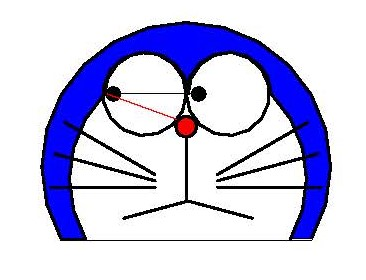
\includegraphics[scale=.3]{doraemon1.jpg}}
        }
    }
    \hfill
    \fbox{
        \subfloat[doraemon (3)]{
            \fbox{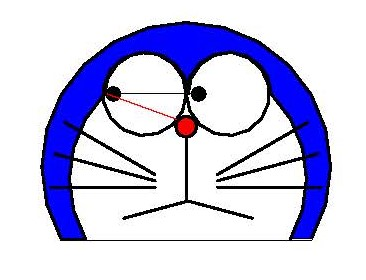
\includegraphics[scale=.5]{doraemon1.jpg}}
        }
    }
    \caption{doraemon\_subfig\_subfloat\_scale}
    \label{14}
\end{figure}

\end{document}